\subsection{Form Clipping}
In Form Clipping we remove the upper and lower part of the image to take the hand written part only.
This done by extracting the edges of the image using Canny edge detection the detect the lines in the edge image using opencv houghlineP function.
After that we only consider the horizontal line that are not at the beginning of the image, sort them, then take the part of the image that lies inside the first and last detected horizontal line.
sample results are shown in Figure \ref{fig:clipping-example} and Figure \ref{fig:clipping-result}.

\begin{figure}[h!]
    \centering
    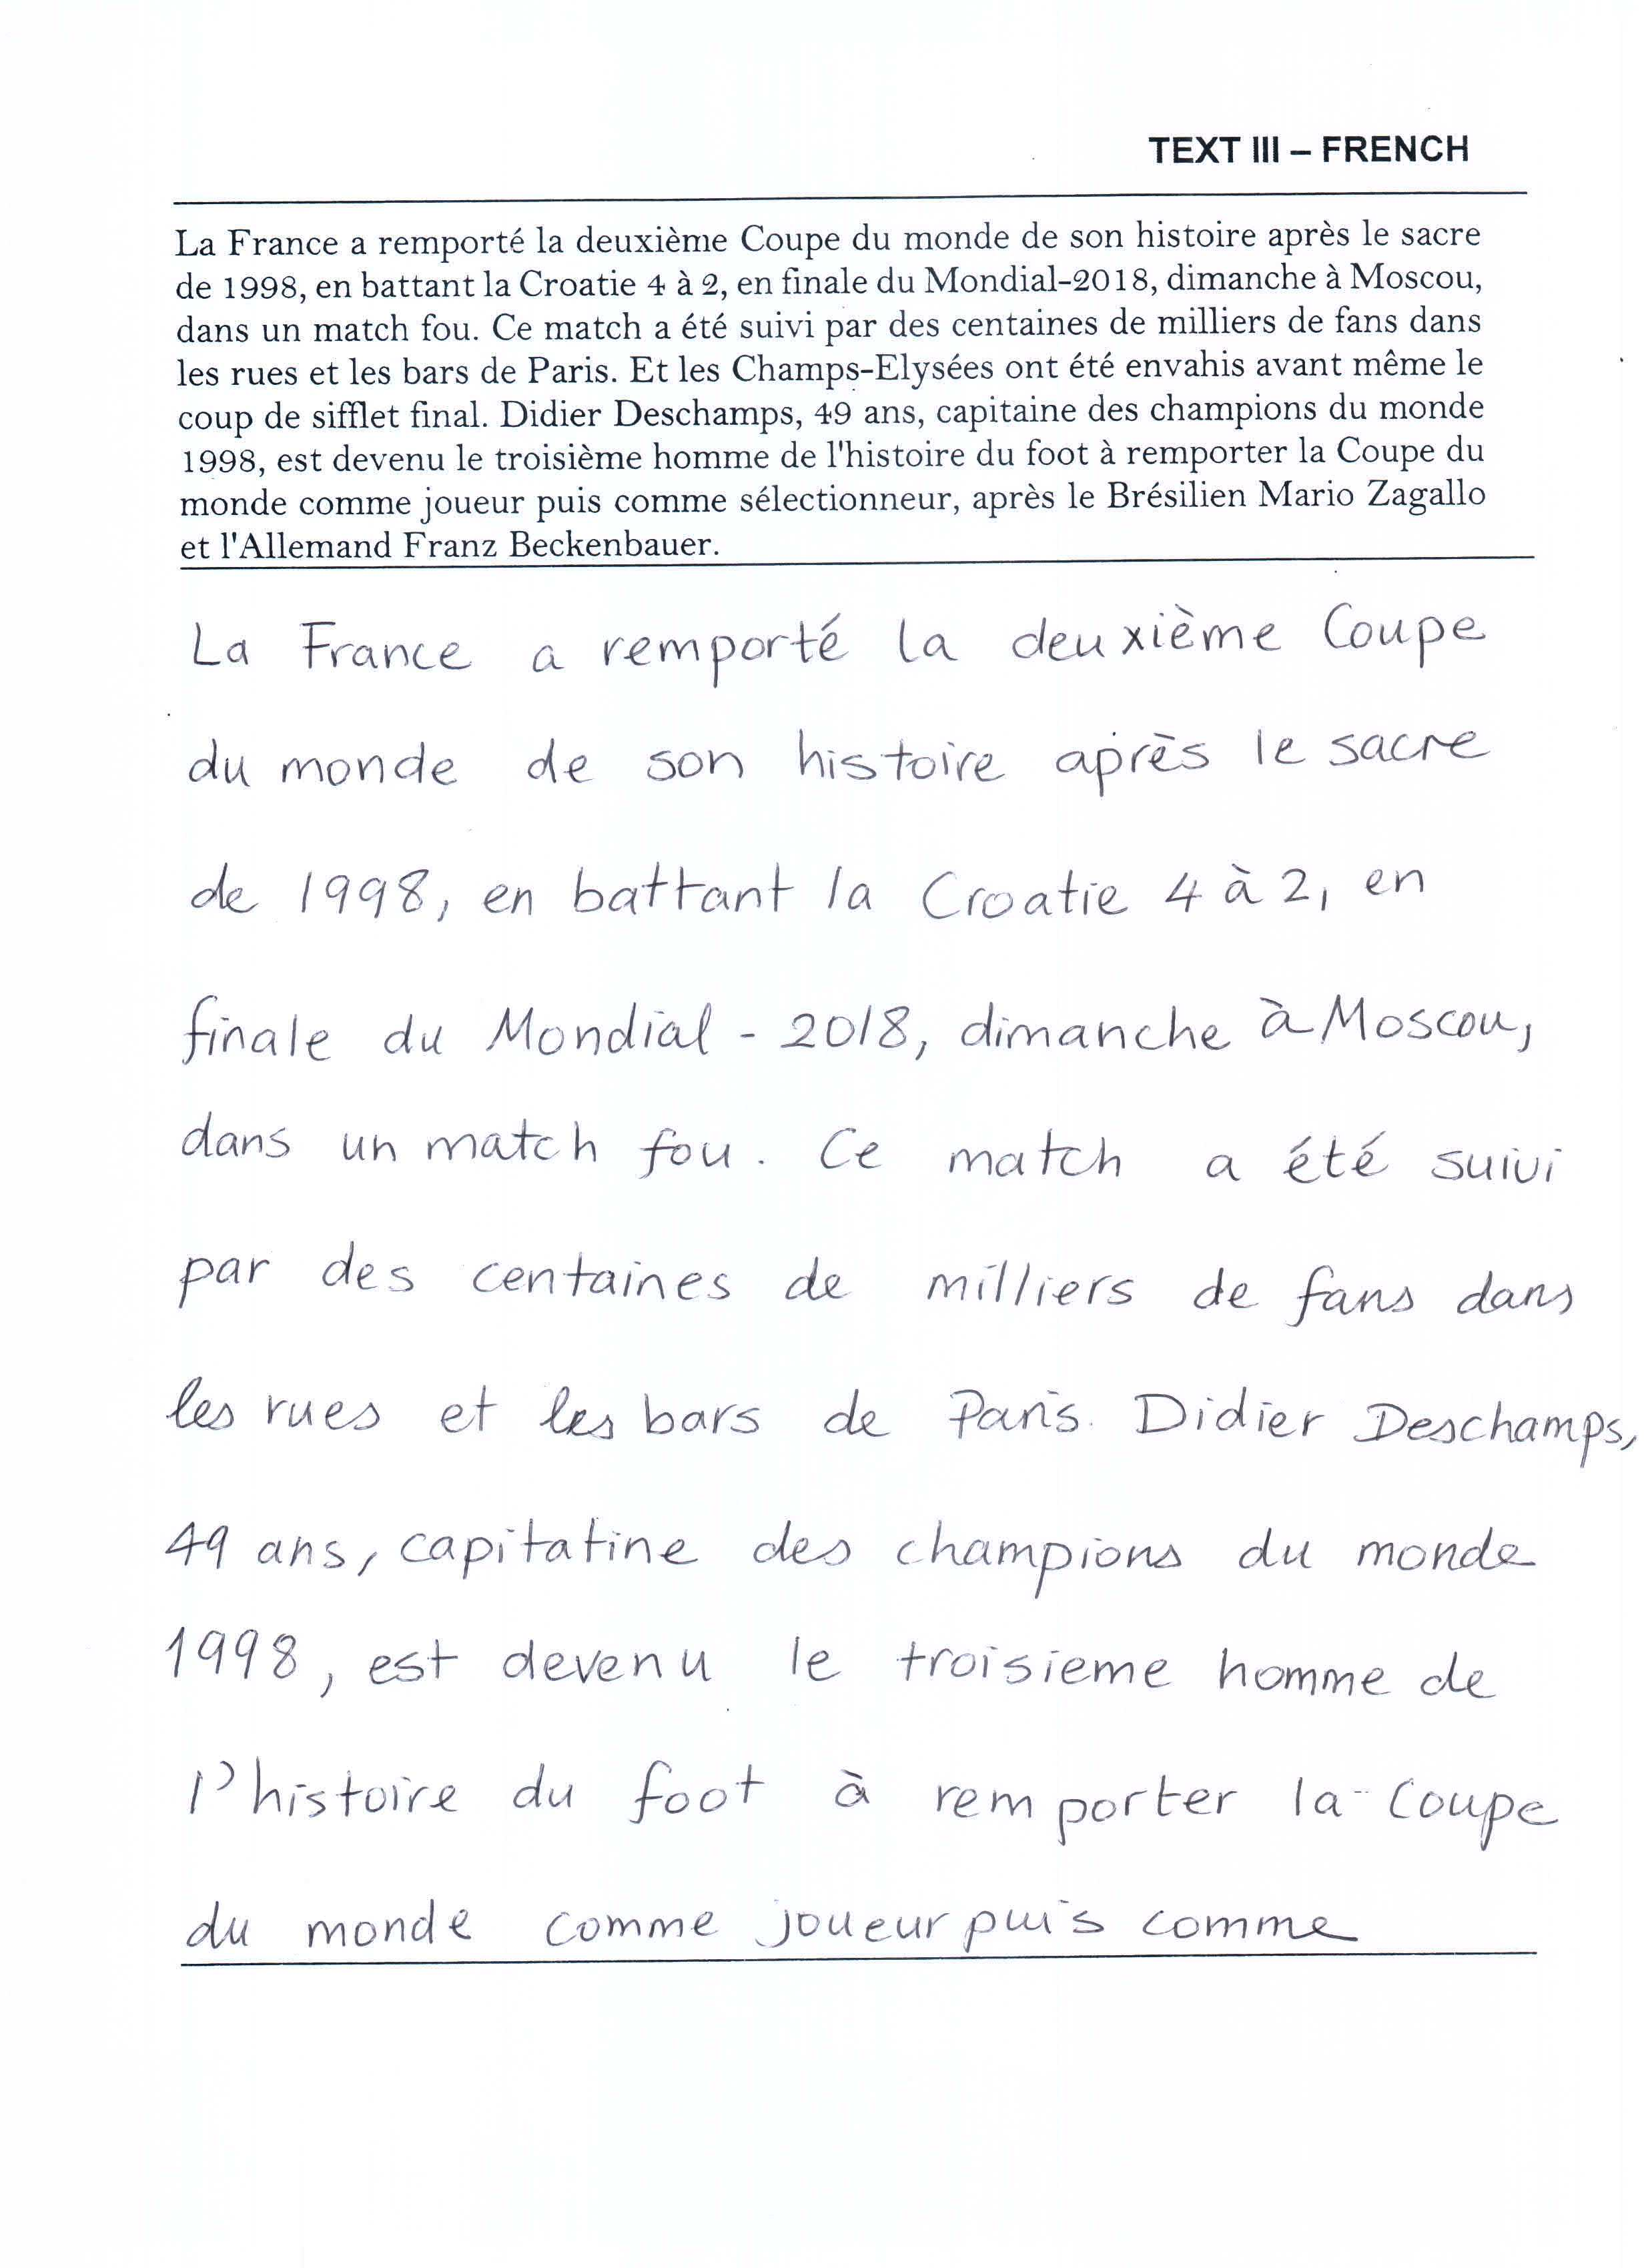
\includegraphics[width=0.4\textwidth]{source/images/5.jpeg}
    \caption{Image before clipping}
    \label{fig:clipping-example}
\end{figure}

\begin{figure}[h!]
    \centering
    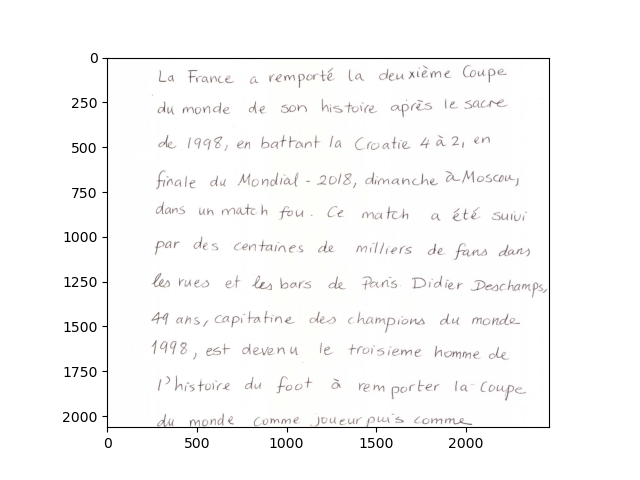
\includegraphics[width=0.4\textwidth]{source/images/img5_result.png}
    \caption{Image after clipping}
    \label{fig:clipping-result}
\end{figure}